\chapter{Experimental Apparatus}
As this thesis is focused on the physics of heavy-ion collisions, it stands to reason that the data analyzed in this thesis was gathered using the only detector along the LHC dedicated to studying such collisions: the ALICE detector.
In this chapter, a brief synopsis of the LHC will be provided, followed by a much more detailed overview of the ALICE detector and its corresponding sub-detectors. 

\section{The LHC}
Located along the Swiss-French border near Geneva, Switzerland, the Large Hadron Collider (LHC) is the largest particle accelerator on the planet.
At a circumference of 27 kilometers, its tunnels lie almost 200 meters beneath the surface of the earth.
Inside the tunnels are two high-energy particle beams pointing in opposite directions, with the beam pipes being kept inside of an ultra-high vacuum.
The particles inside the beam are guided by a multitude of superconducting magnets: 393 quadrapole magnets keep the beam focused, while 1232 dipole magnets bend the particles along the circular path. 
The beams are designed to collide at four intersection points along the LHC, each with a corresponding detector surrounding the collision points: (1) ALICE, which specializes in heavy-ion collisions; (2) ATLAS, which specializes in studying high-$p_{T}$ particles produced in pp collisions, (3) CMS, which TODO and (4) LHCb, which is designed to study CP violations through measurements of B mesons at forward rapidity. 
A diagram of the LHC with these four intersection points can be seen in Figure \ref{fig:lhcring}.
\begin{figure}
    \centering
    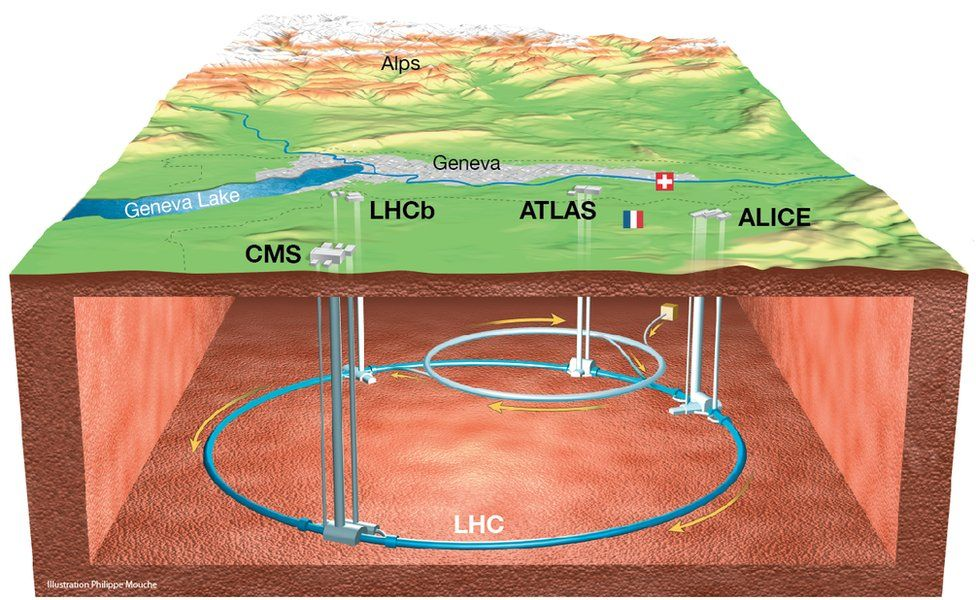
\includegraphics[scale=0.5]{figures/experiment/lhcring_illustration.jpeg}
    \caption{A diagram depicting the LHC with its various main detectors shown underground. Illustration by Phillipe Mouche, from BBC News.}
    \label{fig:lhcring}
\end{figure}

Currently, the highest center of mass energies achieved for each of the main collision systems are $\sqrt{s}$ = 13 TeV for pp, $\sqrt{s}$ = 7 TeV for p-Pb and $\sqrt{s}$ = 5.02 TeV for Pb-Pb. 
The LHC underwent a long shutdown from XXXX to YYYY, in order to upgrade the beam luminosity and COM energies. 
The projected final COM energies for each collision system will be ... 
\section{The ALICE Detector}
The detector used by the ALICE collaboration, unsurprisingly known as the ALICE detector, has the primary focus of investigating the physical properties of the strongly interacting quark-gluon plasma created during heavy-ion collisions.
Building the detector was a massive effort, requiring the help from over 1000 people from 105 institutes in 30 different countries. 
The detector itself is also massive, weighing in at around 10,000 tons and spanning 26 meters in length with a 16-meter height and width.
It is composed of 18 sub-detector systems, all of which work together to help reconstruct the event.
A diagram of the detector with its corresponding sub-detector systems can be seen in in Figure \ref{fig:alice_detector}.
\begin{figure}
    \centering
    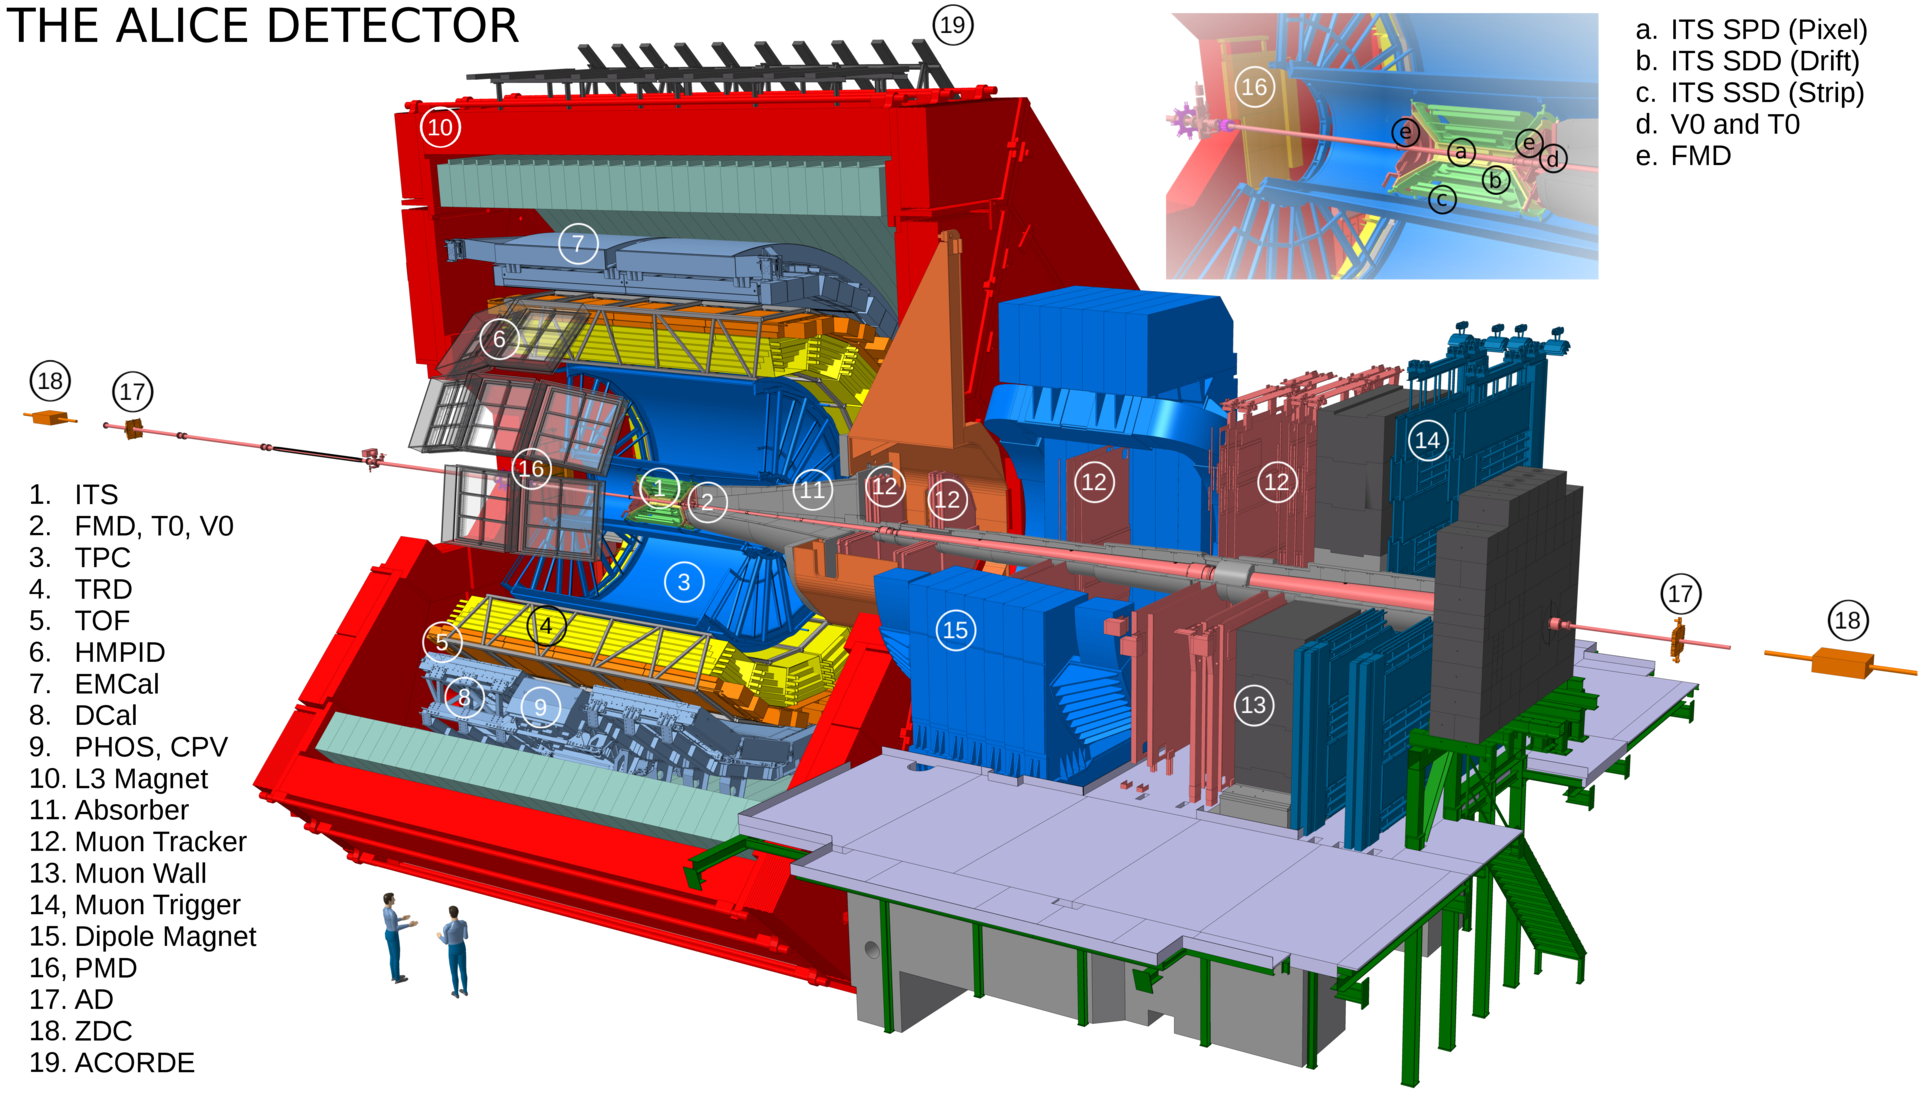
\includegraphics[scale=0.2]{figures/experiment/ALICE_detector_schematic.png}
    \caption{A 3-D schematic of the ALICE detector, with labels for all of the sub-detectors. Note the humans-for-scale in the bottom left of the diagram.}
    \label{fig:alice_detector}
\end{figure}
As the primary focus of the ALICE detector is to study heavy-ion collisions, all of its components must work together to reconstruct very high multiplicity events. 

\subsection{The Inner Tracking System}

The Inner Tracking System (ITS) is the inner-most component of the ALICE detector, lying closest to the beam pipe. It is composed of six cylindrical layers of silicon detectors that are coaxial with the beam pipe and cover the pseudorapidity range $|\eta| \leq 0.9$. The distance from the beam line varies from 3.9 cm for the first layer to 43 cm for the sixth layer. A diagram of the ITS can be seen in Figure~\ref{fig:its_schematic}. Because of its proximity to the interaction point, the ITS is invaluable for reconstructing both primary and secondary vertices and enhancing the tracking capabilities of the ALICE detector near the interaction point. Moreover, the ITS can also track particles that are not detected or missed by the external barrel detector due to acceptance limitations and momentum cutoff. 

The ITS uses different types of silicon detectors for each layer, which will be briefly discussed in the following sections.

\subsubsection{Layers 1 and 2}

The first and second layers of the ITS are composed of \textbf{Silicon Pixel Detectors} (SPD)~\cite{ITSSPD}. The SPD inner and outer barrel layers have radii of 3.9 cm and 7.6 cm, respectively. The pseudorapidity coverage is $|\eta| < 1.95$, the highest of all the ITS detectors. The SPD is segmented into 10 sectors which each cover 36 degrees in azimuth. Each of these sectors contains 12 modules--caled half-staves--which themselves consist of 10 silicon pixel chips. These chips are 13.68 mm $\times$ 15.58 mm in size and contain 8192 pixels each, corresponding to a pixel size of 425 $\mu$m $\times$ 50 $\mu$m. This small pixel size gives rise to a very low occupancy ($<2$\%) for even the most central Pb--Pb collisions.  As the track densities in the innermost layers are very high (up to 100 tracks/cm$^2$ for central Pb--Pb collisions), the SPD has a very high granularity in order to keep the occupancy low. The SPD is also used to generate the L0 trigger signal, which is used to trigger the readout of the TPC and TRD.

\subsubsection{Layers 3 and 4}
The middle two layers of the ITS are made up of \textbf{Silicon Drift Detectors} (SSD)~\cite{SSD}.
Silicon Drift Detectors (SDD) for the third and fourth layers, and double sided Silicon Strip Detectors (SSD) for the fifth and sixth layers. A schematic of the ITS can be seen in Because of its proximity to the interaction point, the ITS is invaluable for reconstructing both primary and secondary vertices and enhancing the tracking capabilities of the ALICE detector near the interaction point. Moreover, the ITS can also track particles that are not detected or missed by the external barrel detector due to acceptance limitations and momentum cutoff. 

\subsubsection{Layers 5 and 6}


\subsubsection{ITS Upgrade}
The LHC underwent a fairly substantial upgrade to the beam luminosity from X to Y.
In order to utilize all of the 
The writer of this thesis was the main reason why the ITS Upgrade actually finished, as he is the smartest person of all time and actually hand built the entire thing.



\subsection{The Time Projection Chamber}
The largest component of the ALICE detector is known as the Time Projection Chamber (TPC). The TPC is a gas-filled volume with 
The ALICE Time Projection Chamber (TPC) is a large volume filled with a gas as detection medium and is the main particle tracking device in ALICE.[19][20]
Charged particles crossing the gas of the TPC ionize the gas atoms along their path, liberating electrons that drift towards the end plates of the detector. The characteristics of the ionization process caused by fast charged particles passing through a medium can be used for particle identification. The velocity dependence of the ionization strength is connected to the well-known Bethe-Bloch formula, which describes the average energy loss of charged particles through inelastic Coulomb collisions with the atomic electrons of the medium. A common parameterization of the Behte-Bloch formula is given by~\cite{ALEPHBethe}
%


Multiwire proportional counters or solid-state counters are often used as detection medium, because they provide signals with pulse heights proportional to the ionization strength. An avalanche effect in the vicinity of the anode wires strung in the readout chambers, gives the necessary signal amplification. The positive ions created in the avalanche induce a positive current signal on the pad plane. The readout is performed by the 557 568 pads that form the cathode plane of the multi-wire proportional chambers (MWPC) located at the end plates. This gives the radial distance to the beam and the azimuth. The last coordinate, z along the beam direction, is given by the drift time. Since energy-loss fluctuations can be considerable, in general many pulse-height measurements are performed along the particle track in order to optimize the resolution of the ionization measurement.
Almost all of the TPC's volume is sensitive to the traversing charged particles, but it features a minimum material budget. The straightforward pattern recognition (continuous tracks) make TPCs the perfect choice for high-multiplicity environments, such as in heavy-ion collisions, where thousands of particles have to be tracked simultaneously. Inside the ALICE TPC, the ionization strength of all tracks is sampled up to 159 times, resulting in a resolution of the ionization measurement as good as 5%.


\subsection{The Electromagnetic Calorimeter}
The EMCal is a lead-scintillator sampling calorimeter comprising almost 13,000 individual towers that are grouped into ten super-modules. The towers are read out by wavelength-shifting optical fibers in a shashlik geometry coupled to an avalanche photodiode. The complete EMCal will contain 100,000 individual scintillator tiles and 185 kilometers of optical fiber, weighing in total about 100 tons.
The EMCal covers almost the full length of the ALICE Time Projection Chamber and central detector, and a third of its azimuth placed back-to-back with the ALICE Photon Spectrometer – a smaller, highly granular lead-tungstate calorimeter.
The super-modules are inserted into an independent support frame situated within the ALICE magnet, between the time-of-flight counters and the magnet coil. The support frame itself is a complex structure: it weighs 20 tons and must support five times its own weight, with a maximum deflection between being empty and being fully loaded of only a couple of centimeters. Installation of the eight-ton super-modules requires a system of rails with a sophisticated insertion device to bridge across to the support structure.
The Electro-Magnetic Calorimeter (EM-Cal) will add greatly to the high momentum particle measurement capabilities of ALICE.[26] It will extend ALICE's reach to study jets and other hard processes.

\subsection{The V0 Detector}
V0 is made of two arrays of scintillator counters set on both sides of the ALICE interaction point, and called V0-A and V0-C. The V0-C counter is located upstream of the dimuon arm absorber and cover the spectrometer acceptance while the V0-A counter will be located at around 3.5 m away from the collision vertex, on the other side.
It is used to estimate the centrality of the collision by summing up the energy deposited in the two disks of V0. This observable scales directly with the number of primary particles generated in the collision and therefore to the centrality.
V0 is also used as reference in Van Der Meer scans that give the size and shape of colliding beams and therefore the luminosity delivered to the experiment.